\documentclass[a4paper,twocolumn,aps,prd,longbibliography,superscriptaddress]{revtex4-1}
%\documentclass[prd,twocolumn,nofootinbib,showpacs]{revtex4-1}

%\usepackage{amsmath,amssymb}
\usepackage{cancel}
\usepackage{graphicx}
%\usepackage{cite}
\usepackage{epsfig}
\usepackage{physics}
\usepackage{amsmath,amsfonts,amssymb}
\usepackage{color,soul}
\newcommand{\myexp}{e^}
\usepackage{float}
\usepackage{graphicx}
\graphicspath{ {Images/} }
\usepackage[utf8]{inputenc}
\usepackage{hyperref}
\usepackage[compatibility=false]{caption}
\usepackage{subcaption}
\usepackage{eurosym}
\usepackage{siunitx}
\usepackage{makecell}
\renewcommand*{\figureautorefname}{FIG.}
\captionsetup[table]{name=TAB.}
\renewcommand*{\tableautorefname}{TAB.}
\renewcommand{\thetable}{\arabic{table}}   
\DeclareSIUnit\year{yr}
\DeclareSIUnit\EUR{\text{\euro}}
\def\bibsection{\section{References}} %remove a linha das referencias
\renewcommand{\andname}{\ignorespaces}

\begin{document}

\title{Sensitivity Analysis on Least-Squares American Options Pricing}

\author{Miguel Ângelo Maia Ribeiro}
\affiliation{Instituto Superior Técnico, Universidade de Lisboa, Portugal}

\author{\\[0.3cm]\small{\textbf{Advisors:} Cláudia Nunes Philippart}}
\affiliation{Instituto Superior Técnico, Universidade de Lisboa, Portugal}
%\\Rui Dilão\\Claude Cochet}
\author{\small{Rui Manuel Agostinho Dilão}}
\affiliation{Instituto Superior Técnico, Universidade de Lisboa, Portugal}
\author{\small{Claude Yves Cochet}}
\affiliation{Global Markets Quantitative Research, BNP Paribas, Portugal}


\begin{abstract}
Derivatives have become increasingly important in recent decades, with the sums currently handled in these markets amounting to over \$542 trillion.
For this reason, it is of the utmost importance to be able to accurately predict the prices of such contracts and be aware of which factors influence them the most.
In this thesis we will study, in particular, the pricing of American options. These contracts are especially difficult to price due to the high uncertainty associated with optimal stopping.
We shall use the procedure proposed by Longstaff and Schwartz to price this type of derivatives. We will, however, make some adjustments in order to better replicate real-world contracts.
Afterwards, we shall perform a variance-based sensitivity analysis, as proposed by Sobol, which provides a measure of how each parameter's uncertainty affects the final option price variance.
This analysis is particularly important in option pricing due to the sometimes-large uncertainty associated with the parameters used in the model, such as the stock price volatility.
% For this reason, we find that the least-squares approach is ideal under such conditions, since we expect it to be less sensitive to volatility than other methods.
\end{abstract}

\maketitle
\section{Introduction}
The stock market has suffered a complete paradigm shift in the past decades. Recent developments in computer science and mathematical finance have greatly enhanced our abilities to predict and take advantage of stock price changes. New forecasting algorithms not only enable us to better defend ourselves against unexpected unfavorable market shifts but even to take advantage of them, making such techniques highly desirable to investors.
With the colossal sums handled daily in the stock market, even a small improvement on the predictive abilities of a given forecasting algorithm can lead to significant increases in profits for investors. In such a highly competitive subject, it should be clear that a lot of resources must be devoted to the research and development of these algorithms. An investor that does not follow this strategy is bound to lose major profits when compared to his better-prepared counterparts.




Along with stock prices, derivatives have also seen great algorithmic developments in recent times. A derivative is simply a contract whose value depends on other simpler financial instruments, such as stocks or interest rates. Derivatives can virtually take any form desirable, so long as there are two parties interested in taking a part in it. In this work, we will focus on the most common type of derivatives~\cite{Hull} - options.

The derivatives market has become increasingly important in recent times~\cite{Hull}. In fact, as of June 2017, derivatives were responsible for over $\$542$ trillion worth of trades, in the Over-the-Counter (OTC) market alone~\cite{BIS}, as can be seen in \autoref{fig:OTC} (the OTC market refers to all deals signed outside of exchanges). Though the market size peaked in 2013 with over $\$710$ trillion, it shrunk in the last decade, due to new regulations implemented after the 2007 global financial crisis~\cite{FT}.

\begin{figure}[H]
    \centering
      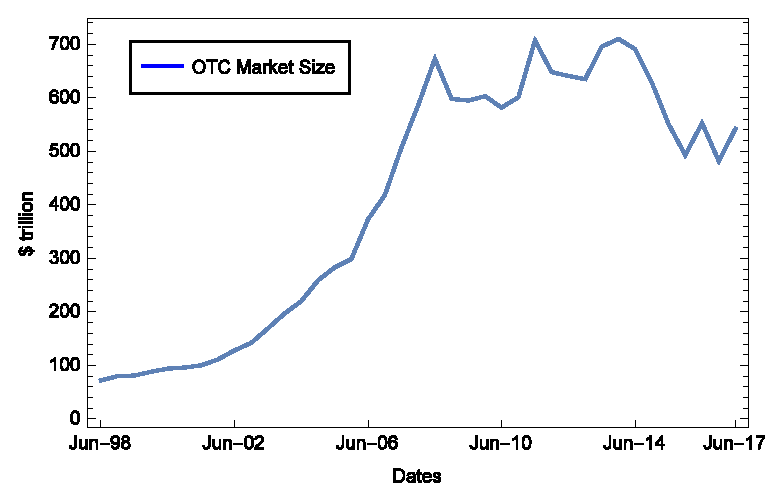
\includegraphics[width=.9\columnwidth,trim={2pt 17pt 0 0},clip]{OTC.eps}
      \caption{Size of OTC derivatives market since May 1996.}\label{fig:OTC}
    \end{figure}

\subsection{Call and Put Options}
Among the many types of derivatives, the most commonly traded are options~\cite{Hull}, of which there are two main types - calls and puts.

In simple terms, a \textit{call option} grants an investor the right to buy the underlying asset (e.g. stock) for a fixed price, known as the \textit{strike price}, by a certain date, known as the \textit{expiration date}.
On the other hand, a \textit{put option} grants an investor the right to sell the underlying asset for the strike price, by the expiration date.

If at the time of exercise, the asset price is above (resp. below) the strike price, we say the option is \textit{in the money} and the owner of a call (resp. put) option should exert his right to buy (resp. sell) the underlying asset, also known as \textit{exercising}, earning the difference between the asset price at the time of exercise and the fixed strike price. Otherwise, if the asset price is below (resp. above) the strike price, we say the option is \textit{out of the money} and it should not be exercised, as this would lead to losses to its owner.

The payoff function of these two types of derivatives can then simply be deduced as
\begin{equation}\label{callput}
\begin{split}
&\text{Payoff}_\text{call}(t)=(S(t)-K)^+;\\
&\text{Payoff}_\text{put}(t)=(K-S(t))^+,
\end{split}
\end{equation}
\noindent where $K$ is the strike price and $S(t)$ is the asset price at the time of exercise, $t$. These functions are represented in \autoref{fig:Payoff}.

\begin{figure}[H]
    \centering
      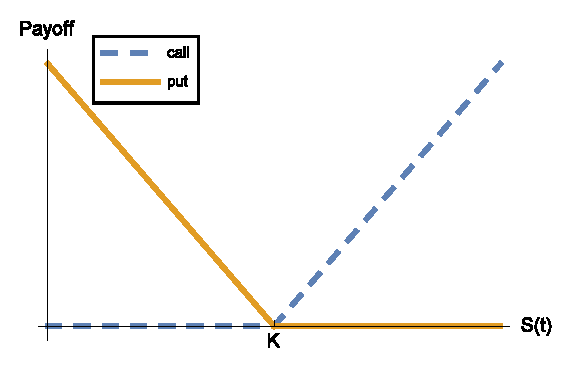
\includegraphics[width=.9\columnwidth]{Payoff.eps}
      \caption{Payoff functions of \textit{call} and \textit{put options}.}\label{fig:Payoff}
    \end{figure}

It's important to note that an option gives the holder the right to buy/sell the underlying asset but he is not obliged to do so. If exercising the option would lead to losses the investor can simply let the option expire. This is one of the most atractive characteristics of options.

In the present work, we shall focus on options whose underlying assets are stocks. Though some of the results presented might also be applied to other option types~\cite{Hull}, these have to be analyzed carefully.


Options have several other advantages that make them especially appealing to investors.
To hedgers (i.e. investors that want to limit their exposure to risk), options provide safety by fixing the future price of a stock i.e. if a hedger is afraid of a future stock price crash in one of the stocks he owns, by buying put options on that same stock, he ensures that his losses are contained because he can always sell the stocks for the fixed strike price, after the stock price crash.
To speculators (i.e. investors that want to take advantage of the uncertainty of future stock prices by betting on their outcome), options grant access to much higher profits i.e. due to the options having a lower price than their underlying stock, a speculator can buy a much larger number of options than stocks with the same initial investment, magnifying the consequences of the outcome: if the speculator's initial prediction proves true, his profits will increase greatly whereas a wrong prediction will lead to a total loss of the initial investment.

Due to all their advantages, and unlike some other types of derivatives, options have a price. Finding the ideal price for an option is quite difficult, however, due to the great complexity of these financial instruments~\cite{Hull}. This is a fundamental concern to investors, since knowing the true value of an option can give them a chance to take advantage of under or overpriced options.




\subsection{European and American Options}
Both call and put options can be further separated into several categories. Among these, European and American options are by far the most commonly traded~\cite{Hull}.

The holder of a \textit{European option} can only exert his right to buy/sell (resp. call/put) the underlying assets at the specified expiration date.
On the other hand, an \textit{American option} enables its owner to exercise it at any time up to its expiration date.



Due to their high importance, options have been studied in detail in the past.
Possibly the most important result in this field came from Fischer Black, Myron Scholes and Robert Merton, who developed a mathematical model to price European options~\cite{Scholes} - the famous Black-Scholes-Merton model - still in use in present days~\cite{Hull}. The last two actually earned the 1997 Nobel prize in Economics for this development.

This model states that a European call or put option's price follows the partial differential equation (PDE)

\begin{equation}\label{BS2}
\pdv{V}{t}+\frac{1}{2}\sigma^2S^2\pdv{V^2}{S^2}+rS\pdv{V}{S}-rV=0,
\end{equation}

\noindent where $V$ is the price of the option, $S$ is the price of the underlying stock, $r$ is the risk-free interest rate and $\sigma$ is the stock price volatility.
Simply put, the volatility of a stock price is a measure of how uncertain the price movement is in the future. A high volatility will lead to great future fluctuations in the stock price.

This model assumes furthermore that stock prices follow a Geometric Brownian Motion (GBM), which can be defined as

\begin{equation}\label{BS}
dS(t)=rS(t)dt+\sigma S(t)dW(t),
\end{equation}
\noindent with $\{W(t),\ t>0\}$ defining a one-dimensional Brownian motion.

Because the stock price depends on a Brownian motion process, it follows that it is not differentiable. For this reason, it's impossible to exactly simulate such a process. An approximation is possible, however, using discrete jumps of length $\Delta t$ and using the Brownian motion property $W(t)\sim \sqrt{t}N(0,1)$~\cite{Mikosch}, with $N(0,1)$ being a normal distribution with 0 expected value and 1 variance.
We can then simply discretize eq. \eqref{BS} into
\begin{equation}
S(t+\Delta t)=S(t)+rS(t)\Delta t+\sqrt{\Delta t}\sigma S(t)N(0,1),
\end{equation}
\noindent where $\Delta t$ corresponds to a given time step. An example of this discretization is represented in \autoref{fig:GBM}.

\begin{figure}[H]
    \centering
      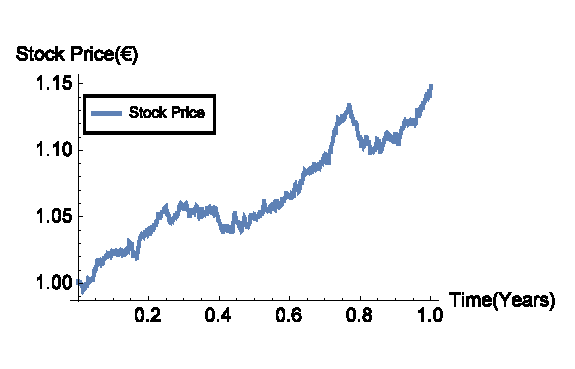
\includegraphics[width=0.9\columnwidth]{GBM.eps}
      \caption{Example of three GBM processes, using the parameters $r=\SI{0.06}{\per\year}$, $\sigma=0.05$, $S(0)=\SI{1}[\EUR]{}$ and time steps $\Delta t=10^{-3}\SI{}{\year}$.}\label{fig:GBM}
    \end{figure}
    
By simulating a large number of paths, some underlying tendencies might become apparent, which will prove useful in option pricing.

Pricing European options is fairly straightforward - we simply need to solve the PDE in eq. \eqref{BS2} in a similar fashion to the initial value problem for the diffusion
equation~\cite{Dilao}. American options, however, pose a much greater challenge.  Unlike European options, no analytic pricing model currently exists for this type of derivatives. Several numerical models have been proposed in the past in an attempt to solve this problem~\cite{Hull}, such as the Longstaff-Schwartz algorithm, which we shall approach in later sections of the present thesis.

Despite their complexity, American options are nonetheless the most currently traded options in exchanges~\cite{Hull}. Thus, it is absolutely critical to understand which variables influence this type of derivatives and by what amount. With this knowledge, one can better defend oneself against market changes and even mitigate potential risks.

\subsection{Sensitivity Analysis}
One of the main difficulties in the study of option pricing arises from the fact that the price of an option is influenced by many factors~\cite{Hull}.
From the strike price to the expiration date, some factors are well defined in the option contract and the investor is well aware of their values. Others, like the stock price volatility or the risk-free interest rate, have an associated uncertainty and require a detailed market study. This input uncertainty will cause a variance in the final model output price.

To fully understand how models with uncertain inputs work, a sensitivity analysis is required. In short, sensitivity analyses indicate which factors have a greater impact on the final model output's variance.
There are many types of sensitivity analyses that go from simple scatter plots~\cite{Saltelli} to more complex Monte-Carlo filtering~\cite{Saltelli}. Variance-based sensitivity analysis is particularly useful when dealing with options.

Initially created by Ilya Sobol in 1990 and later further developed by several people, among which the work by Andrea Saltelli is paramount, variance-based sensitivity analysis enables the knowledge of by how much the final model output's variance would decrease if we could completely nullify the uncertainty of a given input~\cite{Saltelli,Sobol}.

The output variance has contributions from each of the uncertain inputs, as well as their combinations. We can therefore decompose the model output variance, $\mathrm{Var}(Y)$, into each of its components as
\begin{equation}
\mathrm{Var}(Y)=\sum_{i=1}^dV_i+\sum_{i<j}^dV_{ij}+\dots+V_{1\dots d},
\end{equation}
\noindent where $d$ is the total number of uncertain input variables, $V_{i}$ is the contribution of the i\textsuperscript{th} input variable to the total variance, $V_{klm}$ is the combined contribution of the k\textsuperscript{th}, l\textsuperscript{th} and m\textsuperscript{th} variables, and so on.
We can then define the \textit{first order sensitivity index}, $S_i$, as
\begin{equation}\label{Si}
S_i=\frac{V_i}{\mathrm{Var}(Y)},
\end{equation}
\noindent which simply gives the effect in the total output variance when varying only the i\textsuperscript{th} variable.
Furthermore, we can define the \textit{total effect index}, $S_{Ti}$, as
\begin{equation}\label{STi}
S_{Ti}=S_i+\sum_{j}^dS_{ij}+\dots+S_{1\dots d},
\end{equation}
\noindent which can be interpreted as the importance of the i\textsuperscript{th} variable to the total model output variance.
By finding each of these indices we can better understand which variables contribute the most to our uncertainty in the final option price as well as their relationships.

The usefulness of this method in option pricing arises from the fact that if an investor knows where the greatest source of uncertainty of the option price is originated, he can invest greater resources in the mitigation of that uncertainty.
This particular type of sensitivity analysis will be studied in more detail in the later sections of the present work.



\section{Objectives}
In this work, we shall attempt to perform a sensitivity analysis on the price of American options.

As a first step, we will begin by replicating the model developed by Longstaff and Schwartz to price American options.

Having replicated this algorithm, we shall then modify it to more closely resemble real-world stocks.
The model assumes a constant stock price volatility throughout the simulations, which does not hold in the real-world stock market. For this reason, we might implement the GARCH(1,1) model to account for changes in the volatility.
We could also attempt to implement new models for the risk-free interest rate since its value also changes with time.
A further study of which models better suit our needs is still necessary, however, and perfecting the initial algorithm will also be a major section of this thesis.

With the enhanced Longstaff-Schwartz algorithm, we will then apply a variation-based sensitivity analysis, as developed by Sobol and Saltelli.
Some other aspects of this sensitivity analysis will also be considered, such as how each variable's weight changes with time.

Finally, we will try to apply our model to real-world American options.
We shall apply some algorithms, such as the implied volatility model, to obtain some of the required model inputs, like the stock price volatility. The remaining inputs shall be obtained from publicly available data, like the risk-free interest rate.
We will then perform a sensitivity analysis on these results and study them.

\section{State of the art}
\subsection{American Option Pricing}
As previously stated, Longstaff and Schwartz have presented a numerical algorithm to price American options~\cite{Longstaff}.\\
They begin by simulating a very large number (e.g. 100,000) of stock price paths using the PDE in eq. \eqref{BS}. To do so, they partition the option time frame into many (e.g. 50) smaller intervals to simulate each stock price jump, similar to what was presented in \autoref{fig:GBM}. It should be noted that such an approximation no longer perfectly mimics the behavior of an American option since this type of option assumes a continuous exercising time frame. However, a sufficiently great number of partitions would approximate such an option as closely as desired.\\
With the paths simulated, they then check which of the simulated stock price paths are in the money at the time step immediately before expiration. For each of these, they perform a least squares regression - a possible choice of basis functions for the regression is the set of Laguerre polynomials - using the cash flows of immediate exercise against the discounted cash flows of the following time step as data.
With this regression, they obtain a function that returns the expected cash flow of continuation i.e. how much cash flow is a given stock price path expected to generate if it were not immediately exercised.
By comparing the expected cash flow of continuation with the cash flow of immediate exercise, we can check if, for a particular path, whether is optimal to immediately exercise the option or to hold on to the option and then pick the best decision.
This algorithm is then iterated backward through every time step until the present.
Thus, we obtain the expected cash flows of every simulated stock price which we simply need to average over all paths to obtain the American option price.

This algorithm is quite useful and has been shown to give results very similar to other more computationally demanding procedures, such as finite difference~\cite{Longstaff}.

Despite its usefulness, Longstaff and Schwartz's algorithm only uses a simple GBM to describe each of the paths. For this reason, a constant stock price volatility is assumed throughout the simulations, which does not hold in real world stocks.
For this reason, some modifications might be applied to the GBM used in the simulations performed prior to the least-squares section of the algorithm.

One such possible modification is the GARCH(1,1) model for the volatility~\cite{Wei} (short for Generalized Autoregressive Conditional Heteroscedasticity).
It states that the volatility in each stock price path has to be updated after each time step using the formula
\begin{equation}
\sigma_n^2=\gamma V_L+\alpha u_{n-1}^2+\beta\sigma_{n-1}^2,
\end{equation}
\noindent where $\gamma$, $\alpha$ and $\beta$ are weights (summing to unity), $V_L$ corresponds to the long-run average variance, $\sigma_i$ corresponds to the volatility at time step $i$ and $u_i$ follows
\begin{equation}
u_i=\frac{S_i-S_{i-1}}{S_{i-1}},
\end{equation}
\noindent with $S_j$ the stock price at time step $j$.
This model assumes that the volatility increases when great changes in the daily stock price occur and that it decreases otherwise. Furthermore, the long-run average variance, $V_L$, can be deduced from past data and makes the volatilities tend to a constant value.
The GARCH(1,1) is by far the most used of the GARCH($p,q$) models, that depend on the $p$ most recent values of $u_n$ and on the $q$ most recent estimates of $\sigma_n$~\citep{Hull}.

The GARCH(1,1) model provides a better representation of volatilities than the simple assumption that they are constant. Due to its simplicity, it is also easily implemented with negligible computational impact in the calculation of the option prices.

Besides changing over time, the volatility of a stock price is also difficult to estimate. Some methods have been developed in an attempt to solve this problem. One such method is the \textit{implied volatility}. In short, this model outputs the volatility that would be required for an option pricing model (e.g. Black-Scholes method) to return a price equal to the option's market price.
We thus try to find the implied volatility, $\widetilde{\sigma}$, that is a solution to the problem
\begin{equation}
f(\widetilde{\sigma},\cdot)-P=0,
\end{equation}
\noindent where $f(\widetilde{\sigma},.)$ is the price output by the pricing model and $P$ is the option's market price.
Because this problem has no analytical solution, we must use a numerical method to solve it, such as Newton's method.
With this result we can deduce the volatility of the underlying stock price from publicly available option prices.


\subsection{Variance-Based Sensitivity Analysis}
The algorithm developed by Ilya Sobol~\cite{Sobol} to calculate the indices in eqs. \eqref{Si} and \eqref{STi} consists of simply generating two matrices, $\mathbf{A}$ and $\mathbf{B}$, of size $N\times k$, with each of their $N$ rows corresponding to a random extraction from the known distributions of the $k$ uncertain input variables.
A set of $k$ new matrices, $\{\mathbf{C}^{(i)},\ i=1,\dots,k\}$, is then generated, each of these matrices being equal to matrix $\mathbf{A}$ with its i\textsuperscript{th} column replaced by matrix $\mathbf{B}$'s. Refer to the scheme below as an example of these matrices.

\begin{equation*}
\begin{split}
\mathbf{A}&=
 \begin{bmatrix}
  0.500 & 0.500 & 0.500 \\
  0.250 & 0.750 & 0.250 \\
  0.750 & 0.250  & 0.750 \\
  0.125 & 0.625 & 0.875 
 \end{bmatrix},\ \mathbf{B}=\begin{bmatrix}
  0.500 & 0.500 & 0.500 \\
  0.750 & 0.250 & 0.750 \\
  0.250 & 0.750  & 0.250 \\
  0.875 & 0.625 & 0.125 
 \end{bmatrix}\\
 \mathbf{C}^{(1)}&=
 \begin{bmatrix}
  0.500 & 0.500 & 0.500 \\
  0.750 & 0.750 & 0.250 \\
  0.250 & 0.250  & 0.750 \\
  0.875 & 0.625 & 0.875  
  \end{bmatrix}\\
 \mathbf{C}^{(2)}&=
 \begin{bmatrix}
  0.500 & 0.500 & 0.500 \\
  0.250 & 0.250 & 0.250 \\
  0.750 & 0.750  & 0.750 \\
  0.125 & 0.625 & 0.875  
  \end{bmatrix}\\
  \mathbf{C}^{(3)}&=
 \begin{bmatrix}
  0.500 & 0.500 & 0.500 \\
  0.250 & 0.750 & 0.750 \\
  0.750 & 0.250  & 0.250 \\
  0.125 & 0.625 & 0.125 
   \end{bmatrix}
 \end{split}
\end{equation*}

Each of the rows of each of these matrices is then used as input for our pricing model - vectors $f(\mathbf{A})$, $f(\mathbf{B})$ and $\{f(\mathbf{C}^{(i)}),\ i=1,\dots,k\}$ are produced, with each of their entries corresponding to the output of the model using the respective matrix's row.

Having obtained all the vectors, we can use the formulas proposed by Saltelli~\cite{Saltelli} to calculate the indices
\begin{equation}\label{Si2}
S_i=\frac{(1/N)\sum_{j=1}^Nf(\mathbf{B})_j.f(\mathbf{C}^{(i)})_j-f_0^2}{(1/N)\sum_{j=1}^N\left(f(\mathbf{B})_j\right)^2-f_0^2};
\end{equation}
\begin{equation}\label{STi2}
S_{Ti}=1-\frac{(1/N)\sum_{j=1}^Nf(\mathbf{A})_j.f(\mathbf{C}^{(i)})_j-f_0^2}{(1/N)\sum_{j=1}^N\left(f(\mathbf{B})_j\right)^2-f_0^2},
\end{equation}
\noindent where $f(\mathbf{B})_j$, $f(\mathbf{C}^{(i)})_j$ and $f(\mathbf{A})_j$ are the j\textsuperscript{th} entries of the vectors $f(\mathbf{B})$, $f(\mathbf{C}^{(i)})$ and $f(\mathbf{A})$, respectively, and $f_0$ is given by
\begin{equation}
f_0=\frac{1}{N}\sum_{j=1}^Nf(\mathbf{B})_j.
\end{equation}

An empirical explanation of eq. \eqref{Si2} can be obtained by the relation between vectors $f(\mathbf{C}^{(i)})$ and $f(\mathbf{B})$. Because they share the i\textsuperscript{th} variable as input, if this variable has a large influence on the output result, then vectors $f(\mathbf{C}^{(i)})$ and $f(\mathbf{B})$ would be very similar. For this reason, high (or low) values of $f(\mathbf{B})_j$ would be multiplied by high (or low) values of $f(\mathbf{C}^{(i)})_j$, we would have a large scalar product and therefore a large value for $S_i$. On the other hand, if this input variable has little effect on the output, $f(\mathbf{B})_j$ and $f(\mathbf{C}^{(i)})_j$ would be randomly associated and a small $S_i$ would be obtained.
As for eq. \eqref{STi2} a similar explanation can be found. Because $f(\mathbf{A})$ and $f(\mathbf{C}^{(i)})$ share all the inputs but the i\textsuperscript{th}, the scalar product between $f(\mathbf{A})_j$ and $f(\mathbf{C}^{(i)})_j$ would return the first order effect of all input variables but the shared i\textsuperscript{th}. Using the same line of thought as for eq \eqref{Si2}, we are left with a value proportional to the influence of the i\textsuperscript{th} variable in the output.

Having obtained the values for all variable indices, the results can now be interpreted and conclusions can be extracted from them.

\section{Preliminary Work}
Due to its high importance in the development of the sensitivity analysis, the Longstaff-Schwartz algorithm has already been implemented. The results obtained closely resemble the ones presented in the original article~\cite{Longstaff}, as can be seen on \autoref{tab:LS}.

\begin{table}[H]
\centering
\begin{tabular}{|c|c|c|c|c|}
\hline
$S(0)($\euro$)$ & $\sigma$ & $T(\SI{}{\year})$ & \thead{Original\\price$($\euro$)$} & \thead{Replicated\\price$($\euro$)$} \\ \hline
36 & 0.2 & 1 & 4.472 &4.455  \\ \hline
36 & 0.2 & 2 & 4.821 &4.784  \\ \hline
36 & 0.4 & 1 & 7.091 &6.688  \\ \hline
36 & 0.4 & 2 & 8.488 &7.867  \\ \hline
40 & 0.2 & 1 & 2.313 &2.285  \\ \hline
40 & 0.2 & 2 & 2.879 &2.810  \\ \hline
40 & 0.4 & 1 & 5.308 &5.013  \\ \hline
40 & 0.4 & 2 & 6.921 &6.386  \\ \hline
\end{tabular}
\caption{Comparison between the prices provided by Longstaff and Schwartz in their original article and the results obtained from the replicated algorithm, developed for this work. We assumed an American put option with strike price $K=\SI{40}[\EUR]{}$ and an interest rate $r=\SI{0.06}{\per\year}$. A number of 100,000 paths were simulated, each with 50 time steps.}
\label{tab:LS}
\end{table}

\section{Commented Bibliography}
\subsection{Miscellaneous Topics}

John Hull's book is a great source for most option related information. In it, Hull covers most option market mechanics as well as some other recent results in this field in a clear and intuitive way.
In what concerns the present work, the most important state-of-the-art topic explored in the book is related to the GARCH(1,1) model.
\begin{itemize}
\item J. Hull. \textit{Options, Futures, and Other Derivatives}. Boston: Prentice Hall, 2012.
\end{itemize}

\subsection{American Option Pricing}
Longstaff and Schwartz's paper on the pricing of American options will be heavily used throughout this work. Most results will be based on some variation of their algorithm. Their paper is not only important for the results it presents but also for the examples it provides that enable a clear and deep understanding of the algorithm.
\begin{itemize}
\item  F. Longstaff and E. Schwartz. \textit{Valuing American Options by Simulation: a Simple Least-Squares Approach}. The review of financial studies, 14(1):113–147, 2001.
\end{itemize}

Chloe's book presents some useful algorithms in the derivatives field. Though Chloe presents no new results in the option pricing field, some of the simulations developed in this thesis may be based, up to some extent, in the ones presented in the book.
\begin{itemize}
\item G. H. Choe. \textit{Stochastic Analysis for Finance with Simulations}. Springer International Publishing, 2016.
\end{itemize}

\subsection{Sensitivity Analysis}
Saltelli's book provides a deep insight into sensitivity analysis. In particular, it gives a great explanation of the variance-based sensitivity analysis used in the present work as well as all the necessary background.
\begin{itemize}
\item A. Saltelli et al. \textit{Global Sensitivity Analysis: The Primer}. John Wiley, 2008.
\end{itemize}

\section{Timetable}
\begin{enumerate}
\item Time series analysis of expired American put options. (1 month)
\item Development of the algorithms for the variance-based sensitivity analysis with respect to the volatility, interest rate and initial stock price. (2.5 months)
\item Improvement of the Longstaff-Schwartz algorithm. (1.5 months)
\begin{itemize}
\item Research of recent developments in the stock price simulation field.
\item Implementation of the GARCH(1,1) model for the volatility.
\item Implementation of the implied volatility model.
\item Implementation of new methods found.
\end{itemize}
\item Writing of the thesis. (1 month)
\end{enumerate}


\bibliographystyle{abbrv}
\bibliography{Thesis}


\end{document}


\iffalse
\section{Thesis Supervisors}
\begin{itemize}
  \item Cláudia Nunes Philippart, \ \ cnunes@math.tecnico.ulisboa.pt
  \item Rui Manuel Agostinho Dilão, \ \ ruidilao@tecnico.ulisboa.pt
  \item Claude Yves Cochet, \ \ claude.cochet@bnpparibas.com
\end{itemize}
\fi


\iffalse
Among these, the most commonly traded are call and put options. In short, a call (resp. put) option gives an investor the right to buy (resp. sell) a particular stock for a fixed price (called the strike price) at some point in the future. If the stock price increases above (resp. decreases below) the fixed price, the investor can simply buy the said stock in the stock market for the lower fixed (resp. current) price, and sell it immediately after for the higher current (resp. fixed) price, earning the difference. If, otherwise, the stock price goes down (resp. up), then the option is worthless and the investor loses his investment.\\
The payoff functions can be easily deduced as
\begin{equation}\label{callput}
\begin{split}

\end{split}
\end{equation}
\noindent where $K$ is the strike price and $S(t)$ is the stock price at the time of exercise, $t$.\fi
\iffalse
In short, options magnify consequences: a good forecast turns into a large profit whereas a bad prediction results in a loss of investment.
\fi
\iffalse
For one, they limit the exposure to risk, e.g. if the price of a given stock were to crash, stock holders would lose a serious amount of funds whereas the owner of a call option would only lose his smaller original investment. On the other hand, options can also lead to greater profits e.g. using the same example of the stock price crash, the owner of a put option could buy this option for the lower current price (after the crash) and sell it for the higher price, fixed at the time of acquisition, before the crash happened.

This type of derivatives also comes with its own caveats. The main disadvantage is the fact that options always deal with stock prices in the future, i.e one can never precisely anticipate how much will be earned, if anything at all. Thus, it's clear that accurately modeling the stock price is paramount when dealing with options.
\fi
\iffalse
Call and put options are also divided into different types. The two most commonly used are European and American options. a European option can only be exercised - buying/selling the stocks for the fixed stock price with a call/put option - at a fixed date in the future, whereas an American option can be exercised anytime up until that fixed date. The payoffs of each of these types of options is simply
\begin{equation}
\begin{split}
&\text{Payoff}_\text{European}=\text{Payoff}_\text{call/put}(T);\\
&\text{Payoff}_\text{American}=\text{Payoff}_\text{call/put}(t), \ \ \ \forall 0<t<T,
\end{split}
\end{equation}

\noindent where $\text{Payoff}_\text{call/put}(t)$ corresponds to the payoffs from equations \eqref{callput} and $T$ corresponds the fixed exercise date of European options.
\fi
\iffalse
When dealing with problems with no analytic solutions, such as the case of American options pricing, it becomes impossible to precisely predict how the model inputs directly affect the final output.

When dealing with inputs with an associated uncertainty, one must use sensitivity analysis to find how the model parameters influence the final result.

A sensitivity analysis simply outputs

Many factors have a weight in the final price of an option.
Because there is no analytic solution to price American options, we depend solely on numerical models to achieve this task.
\fi
\iffalse
First we will begin by simulating a large number of stocks, using the simple Black-Scholes formula to generate each path. The main point behind this method is to apply the Monte Carlo approach to the stock price which will be used later in the option pricing.
After generating all the paths, we shall attempt to replicate the method developed by Longstaff and Schwartz for pricing American options, using the results from the previous simulation.
Next, we will modify the initial simulations using more complex models that better replicate real-world stocks, such as varying volatility, varying interest rate. We shall further study which other factors influence the final price of an option.
We shall then apply a sensitivity analysis on the option price, using the model developed by Sobol and Saltelli.
\fi
\iffalse

\noindent Derivatives have become increasingly important in recent decades, with the sums currently handled in these markets amounting to several trillion dollars.\\
For this reason, it is of the utmost importance to be able to accurately predict the payoff of such contracts to correctly price them.\\
In this thesis we will study particularly the pricing of American options. These contracts are especially difficult to price due to the high uncertainty associated with optimal stopping.\\
Several methods have been suggested to achieve this goal, such as finite difference, but we shall use the procedure proposed by Longstaff et al., using Monte Carlo simulation and least-squares regression.\\
We will mainly focus on the sensitivity analysis of this pricing process, namely how the parameters’ volatility affects the final calculated price.\\
This analysis is particularly important due to the sometimes-large uncertainty associated with the parameters used. For this reason, we find that the least-squares approach is ideal under such conditions, since we expect it to be less sensitive to volatility than other methods.
\fi

\iffalse
\begin{table}[H]
\centering
\begin{tabular}{|c|c|c|c|c|}
\hline
\textbf{$S(0)$}$($\euro$)$ & \textbf{$\sigma$} & \textbf{$T$}$(\SI{}{\year})$ & \thead{\textbf{Original}\\\textbf{price}$($\euro$)$} & \thead{\textbf{Replicated}\\\textbf{price}$($\euro$)$} \\ \hline
36 & 0.2 & 1 & 4.472$\pm$0.010 &4.455  \\ \hline
36 & 0.2 & 2 & 4.821$\pm$0.012 &4.784  \\ \hline
36 & 0.4 & 1 & 7.091$\pm$0.020 &6.688  \\ \hline
36 & 0.4 & 2 & 8.488$\pm$0.024 &7.867  \\ \hline
40 & 0.2 & 1 & 2.313$\pm$0.009 &2.285  \\ \hline
40 & 0.2 & 2 & 2.879$\pm$0.010 &2.810  \\ \hline
40 & 0.4 & 1 & 5.308$\pm$0.018 &5.013  \\ \hline
40 & 0.4 & 2 & 6.921$\pm$0.022 &6.386  \\ \hline
\end{tabular}
\caption{My caption}
\label{tab:LS}
\end{table}
\fi

\iffalse
The algorithm developed by Ilya Sobol~\cite{Sobol} to calculate the indices in eqs. \eqref{Si} and \eqref{STi} consists of simply generating two vectors, $A$ and $B$, of size $N$, with each of their entries corresponding to a single model run with a random trial of the uncertain input variables over their known distributions.
A set of new vectors, $A^{(i)}$, is then generated using the same input values used to generate vector $A$ but replacing the values of the i\textsuperscript{th} input variable with the values used in vector $B$. Thus, we should generate one vector $C^{(i)}$ for each of the input variables with associated uncertainty.

Having obtained all the vectors, we can use the formulas proposed by Saltelli~\cite{Saltelli2} to calculate the indices
\begin{equation}\label{Si3}
S_i\approx\frac{1}{N\mathrm{Var}(Y)}\sum_{j=1}^NB_j\left(C^{(i)}_j-A_j\right);
\end{equation}
\begin{equation}\label{STi3}
S_{Ti}\approx\frac{1}{2N\mathrm{Var}(Y)}\sum_{j=1}^N\left(C^{(i)}_j-A_j\right)^2,
\end{equation}
\noindent where $B_j$, $C^{(i)}_j$ and $A_j$ are the j\textsuperscript{th} entries of the vectors $B$, $C^{(i)}$ and $A$, respectively.


The concept behind eq. \eqref{Si2} is related to the high correlation between vectors $C^{(i)}$ and $B$. If the i\textsuperscript{th} variable has a large influence on the output variance then, whenever $C^{(i)}_j$ is large, $B_j$ would also be large, because they share the same i\textsuperscript{th} input variable. The value of $A_j$, however, would be independent of $B_j$. When multiplying $C^{(i)}_j$ by $B_j$ on eq. \eqref{Si2}, the highly correlated values would return a larger result than the uncorrelated multiplication of $A_j$ and $B_j$. After the subtraction, we would be left with a large value for $S_i$.
On the other hand, if the i\textsuperscript{th} variable has little or no influence on the model output, the values $C^{(i)}_j$ would be uncorrelated with $B_j$ and would vanish after the subtraction. Thus, the value of $S_i$ would be small.
As for eq. \eqref{STi2}, it is clear that the vectors $A$ and $C^{(i)}$ have the same input variables except for the i\textsuperscript{th} variable. Thus, if this variable has a great influence in the model output, even small differences in this input will cause $A_j$ and $C^{(i)}_j$ to be very distinct. On the other hand, if this input has little impact in the model output, $A_j$ and $C^{(i)}_j$ would be very similar.
By squaring the difference, we obtain a measure of how distinct these vectors are and thus how influential is the i\textsuperscript{th} variable.
\fi

\iffalse
\begin{equation}\label{Si2}
S_i\approx\frac{1}{N\mathrm{Var}(Y)}\sum_{j=1}^Nf(\mathbf{B})_j\left(f(\mathbf{C}^{(i)})_j-f(\mathbf{A})_j\right);
\end{equation}
\begin{equation}\label{STi2}
S_{Ti}\approx\frac{1}{2N\mathrm{Var}(Y)}\sum_{j=1}^N\left(f(\mathbf{C}^{(i)})_j-f(\mathbf{A})_j\right)^2,
\end{equation}
\fi

\iffalse
After the division, we would be left with an index $S_i$ very close to 1. The value of $f(\mathbf{A})_j$, however, would be independent of $f(\mathbf{B})_j$. When multiplying $f(\mathbf{C}^{(i)})_j$ by $f(\mathbf{B})_j$ on eq. \eqref{Si2}, the highly correlated values would return a larger result than the uncorrelated multiplication of $f(\mathbf{A})_j$ and $f(\mathbf{B})_j$. After the subtraction, we would be left with a large value for $S_i$.
On the other hand, if the i\textsuperscript{th} variable has little influence on the model output, the values $f(\mathbf{C}^{(i)})_j$ would be barelly correlated with $f(\mathbf{B})_j$ and would vanish after the subtraction. Thus, the value of $S_i$ would be small.
As for eq. \eqref{STi2}, it is clear that the vectors $f(\mathbf{A})$ and $f(\mathbf{C}^{(i)})$ have the same input variables except for the i\textsuperscript{th} variable. Thus, if this variable has a great influence in the model output, even small differences in this input will cause $f(\mathbf{A})_j$ and $f(\mathbf{C}^{(i)})_j$ to be very distinct. On the other hand, if this input has little impact in the model output, $f(\mathbf{A})_j$ and $f(\mathbf{C}^{(i)})_j$ would be very similar.
By squaring the difference, we obtain a measure of how distinct these vectors are and thus how influential is the i\textsuperscript{th} variable.
\fi